\section{Classical Wave Equation}

\begin{frame}{Approach to the classical wave equation}
    Our first goal is to approximate the solution of

    \begin{equation*}
        \fcolorbox{BrickRed}{white}{$\displaystyle\frac{\partial^2u}{\partial t^2}-c^2\frac{\partial^2u}{\partial x^2}=0$} \ \longleftarrow \ \text{\textbf{\textcolor{BrickRed}{d'Alembert equation}}}
    \end{equation*}

    \vfill

    \pause

    \begin{figure}[H]
    \centering
    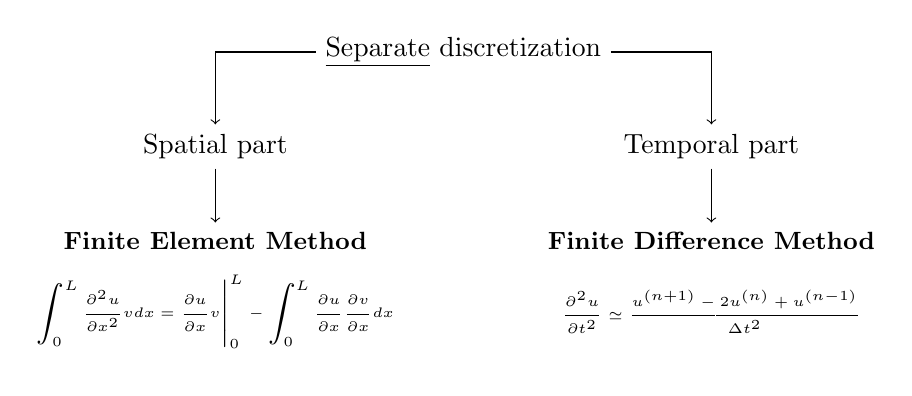
\begin{tikzpicture}
        \node at (0,3) (A) {\underline{Separate} discretization};
        \node at (-3.15,1.8) (B) {Spatial part};
        \node at (3.15,1.8) (C) {Temporal part};
        \node at (-3.15,0.6) (D) {\small{\textbf{Finite Element Method}}};
        \node at (3.15,0.6) (E) {\small{\textbf{Finite Difference Method}}};
        \node at (-3.15,-0.3) (F) {\tiny{$\displaystyle\int_0^L\frac{\partial^2u}{\partial x^2}vdx=\frac{\partial u}{\partial x}v\bigg|_0^L-\int_0^L\frac{\partial u}{\partial x}\frac{\partial v}{\partial x}dx$}};
        \node at (3.15,-0.3) (G) {\tiny{$\displaystyle\frac{\partial^2u}{\partial t^2}\simeq\frac{u^{(n+1)}-2u^{(n)}+u^{(n-1)}}{\Delta t^2}$}};

        \draw[->] (A) -- (-3.15,3) -- (B);
        \draw[->] (A) -- (3.15,3) -- (C);
        \draw[->] (B) -- (D);
        \draw[->] (C) -- (E);

        \draw[white] (3.2,-1) -- (3.2,0);
    \end{tikzpicture}
\end{figure}
\end{frame}

\subsection{Numerical discretization}

\begin{frame}{From PDE to ODEs}
    To do so, a \textbf{separable base} must be chosen:

    \begin{equation*}
        u_h(x,t)=\sum_{j=1}^Nu_j(t)\phi_j(x)
    \end{equation*}

    \vfill

    \pause

    Managing the boundary term separately, the weak formulation goes as

    \small

    \begin{equation*}
        \int_0^L\frac{\partial^2\textcolor{RoyalBlue}{u}}{\partial t^2}\textcolor{ForestGreen}{v}dx+c^2\int_0^L\frac{\partial\textcolor{RoyalBlue}{u}}{\partial x}\frac{\partial\textcolor{ForestGreen}{v}}{\partial x}dx=0 \qquad \forall v\in H^1([0,L])
    \end{equation*}

    \pause

    \begin{equation*}
        \Big\Downarrow
    \end{equation*}

    \vspace{-0.35cm}

    \begin{equation*}
        \textcolor{RoyalBlue}{\sum_{j=1}^N}\frac{d^2\textcolor{RoyalBlue}{u_j}}{dt^2}\int_0^L\textcolor{RoyalBlue}{\phi_j}\textcolor{ForestGreen}{\phi_i}dx+c^2\textcolor{RoyalBlue}{\sum_{j=1}^Nu_j}\int_0^L\frac{\partial\textcolor{RoyalBlue}{\phi_j}}{\partial x}\frac{\partial\textcolor{ForestGreen}{\phi_i}}{\partial x}dx=0 \qquad \forall i=1,\dots,N
    \end{equation*}

    \normalsize
\end{frame}

\begin{frame}{Matrix formulation}
    Let's define

    \begin{alignat*}{3}
        M&:M_{i,j}&&=\int_0^L\phi_j\phi_idx \ &&\longleftarrow \ \text{\textbf{\textcolor{BrickRed}{Mass matrix}}}\\
        A&:A_{i,j}&&=\int_0^L\frac{\partial\phi_j}{\partial x}\frac{\partial\phi_i}{\partial x}dx \ &&\longleftarrow \ \text{\textbf{\textcolor{BrickRed}{Stiffness matrix}}}
    \end{alignat*}

    \pause

    \begin{equation*}
        \Big\Downarrow
    \end{equation*}

    \begin{equation*}
        \fcolorbox{BrickRed}{white}{\text{$\displaystyle M\frac{d^2\boldsymbol{u}}{dt^2}+c^2A\boldsymbol{u}=0$}}
    \end{equation*}
\end{frame}

\begin{frame}{Time discretization}
    Let's apply \textbf{\textcolor{BrickRed}{implicit} central difference scheme}:

    \begin{equation*}
        M\frac{\boldsymbol{u}^{(n+1)}-2\boldsymbol{u}^{(n)}+\boldsymbol{u}^{(n-1)}}{\Delta t^2}+c^2A\boldsymbol{u}^{\textcolor{BrickRed}{(n+1)}}=0
    \end{equation*}

    \pause

    \begin{equation*}
        \Big\Downarrow
    \end{equation*}

    \begin{equation*}
        \fcolorbox{BrickRed}{white}{\text{$\displaystyle\left(\frac{1}{\Delta t^2}M+c^2A\right)\boldsymbol{u}^{(n+1)}=\frac{2}{\Delta t^2}M\boldsymbol{u}^{(n)}-\frac{1}{\Delta t^2}M\boldsymbol{u}^{(n-1)}$}}
    \end{equation*}
\end{frame}

\subsection{Results}

\begin{frame}{Analytical solutions}
    Solutions are known since 1747 due to d'Alembert himself.

    \vfill

    \alt<1>{\begin{itemize}
        \item \textbf{Dirichlet} boundary conditions: $\displaystyle u(0,t)=u(L,t)=0$
        
        \vspace{0.1cm}
        
        \begin{equation*}
            \fcolorbox{BrickRed}{white}{\text{$\displaystyle u(x,t)=\sum_{n=1}^\infty A_n\cos\left(\frac{n\pi}{L}ct\right)\sin\left(\frac{n\pi}{L}x\right)$}}
        \end{equation*}

        with $A_n=\frac{2}{L}\int_0^Lf(x)\sin\left(\frac{n\pi}{L}x\right)dx$.

        \vfill

        \begin{figure}[H]
            \centering
            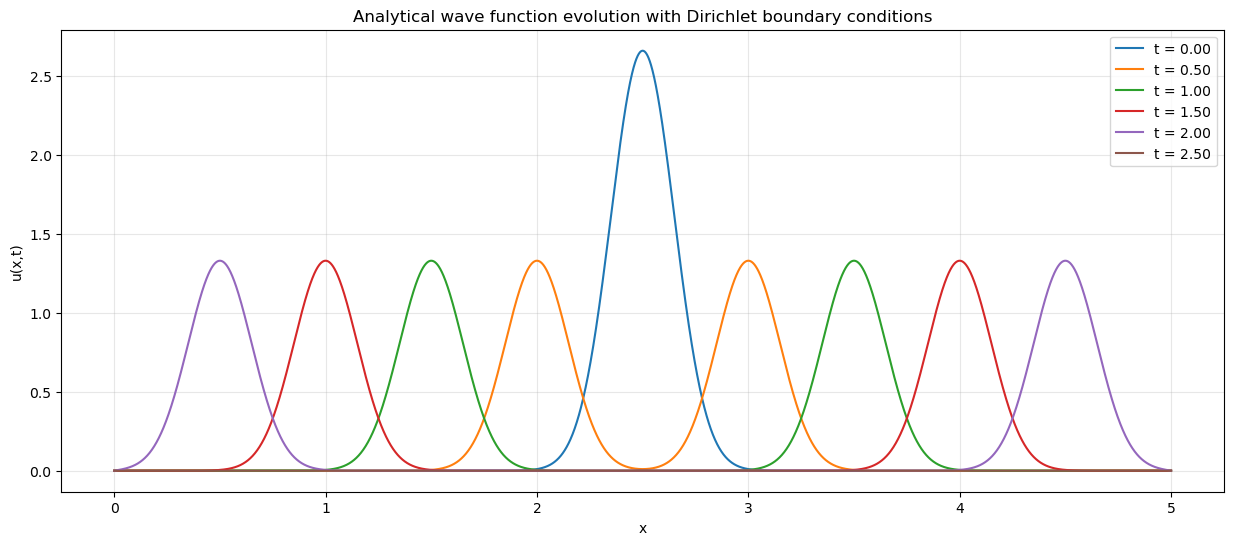
\includegraphics[width=0.8\textwidth]{Immagini/plot-dirichlet-analytical.png}
        \end{figure}
    \end{itemize}}{}

    \alt<2>{\begin{itemize}
        \item \textbf{Neumann} boundary conditions: \small{$\displaystyle\frac{\partial u}{\partial x}\bigg|_{x=0}=\frac{\partial u}{\partial x}\bigg|_{x=L}=0$}
        
        \vspace{0.1cm}

        \normalsize
        
        \begin{equation*}
            \fcolorbox{BrickRed}{white}{\text{$\displaystyle u(x,t)=A_0+\sum_{n=1}^\infty A_n\cos\left(\frac{n\pi}{L}ct\right)\cos\left(\frac{n\pi}{L}x\right)$}}
        \end{equation*}

        with $A_0=\frac{1}{L}\int_0^Lf(x)dx$, $A_n=\frac{2}{L}\int_0^Lf(x)\cos\left(\frac{n\pi}{L}x\right)dx$.

        \vfill

        \begin{figure}[H]
            \centering
            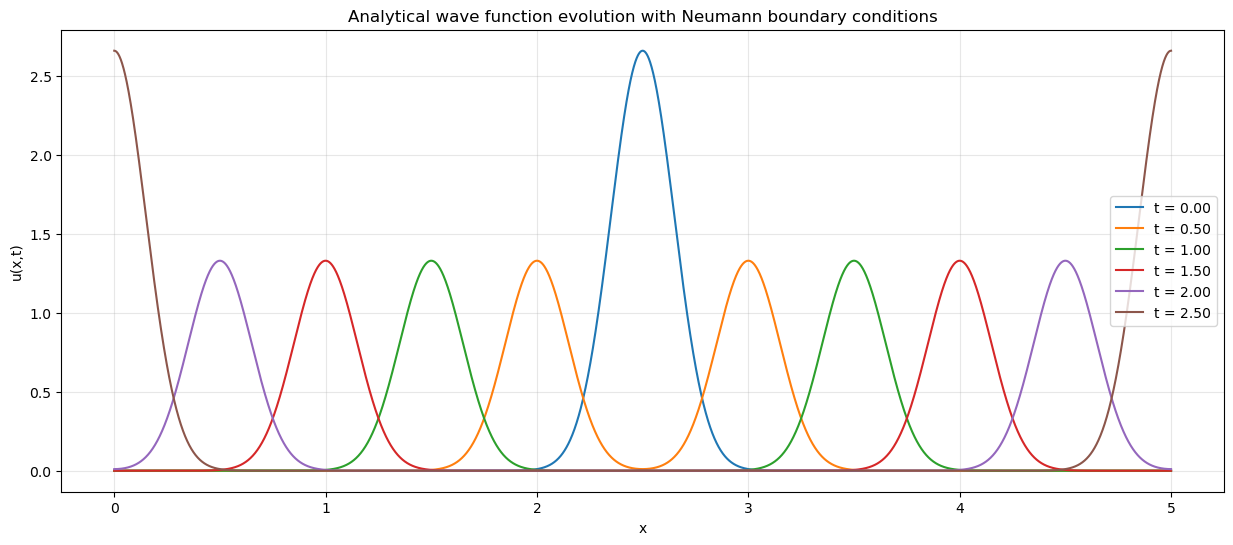
\includegraphics[width=0.8\textwidth]{Immagini/plot-neumann-analytical.png}
        \end{figure}
    \end{itemize}}{}
\end{frame}

\begin{frame}{Approximate solutions}
    \small

    The selection of discretization steps should\normalsize{$^{\boldsymbol{\textcolor{BrickRed}{\ast}}}$} \small{take into account}

    \begin{equation*}
        \text{\textbf{\textcolor{BrickRed}{CFL} stability condition}}: \ \frac{c\Delta t}{\Delta x}\lesssim1
    \end{equation*}

    \small

    \uncover<2>{\begin{center}
        Choosing \underline{first-order Lagrange polynomials} as $\left\{\phi_i\right\}$:
    \end{center}}

    \vfill

    \normalsize

    \visible<2>{\begin{minipage}{0.49\textwidth}
        \begin{center}
            \small{\textbf{Dirichlet}}
        \end{center}

        \vspace{-0.2cm}

        \begin{figure}[H]
            \centering
            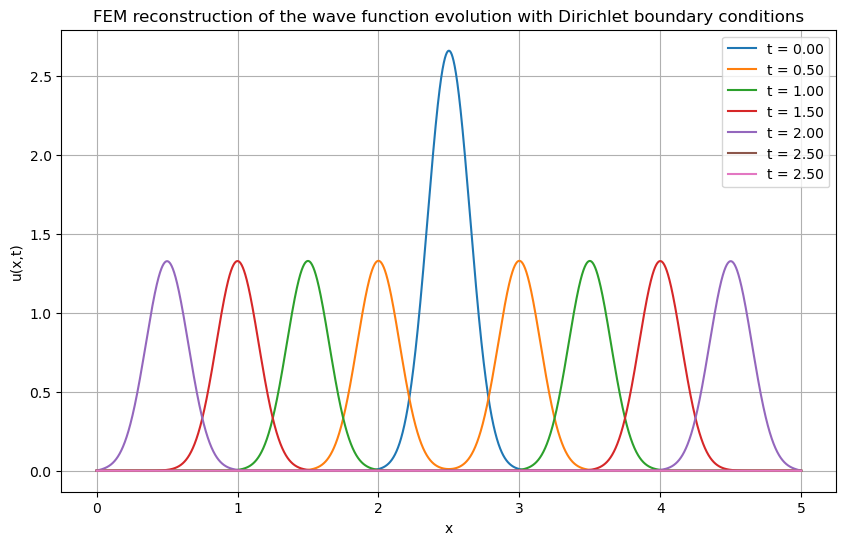
\includegraphics[width=\textwidth]{Immagini/plot-dirichlet-approximated.png}
        \end{figure}
    \end{minipage}
    \hfill
    \begin{minipage}{0.49\textwidth}
        \begin{center}
            \small{\textbf{Neumann}}
        \end{center}

        \vspace{-0.2cm}

        \begin{figure}[H]
            \centering
            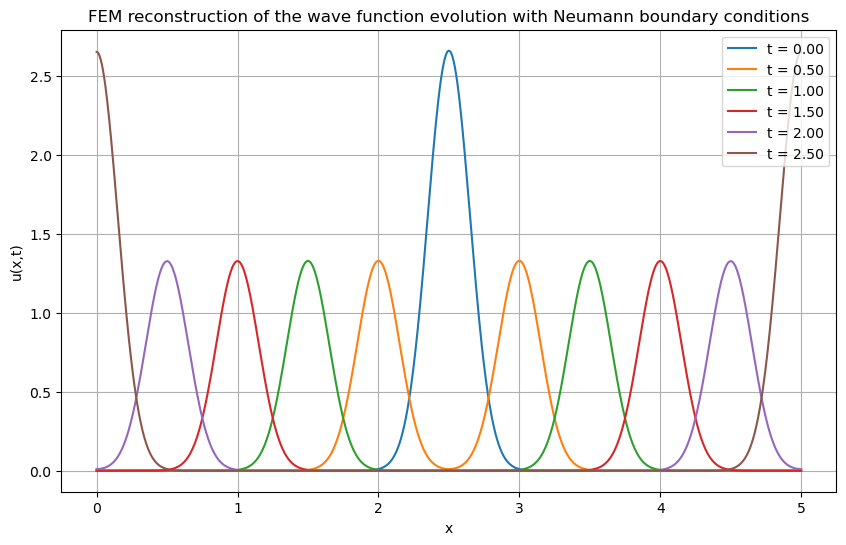
\includegraphics[width=\textwidth]{Immagini/plot-neumann-approximated.png}
        \end{figure}
    \end{minipage}}

    \vfill

    $^{\boldsymbol{\textcolor{BrickRed}{\ast}}}$\scriptsize{While for implicit schemes it is only a recommendation, for explicit ones it is \underline{mandatory}.}

    \normalsize
\end{frame}

\begin{frame}{Energy loss}
    \small

    A strong indicator of numerical correctness is \textbf{\underline{energy conservation}}.

    \pause

    \begin{equation*}
        \text{\textbf{\textcolor{BrickRed}{Energy}}:} \ E=\underbrace{\frac{T}{2c^2}\int_0^L\left(\frac{\partial u}{\partial t}\right)^2dx}_{\text{Kinetic}}+\underbrace{\frac{T}{2}\int_0^L\left(\frac{\partial u}{\partial x}\right)^2dx}_{\text{Potential}}
    \end{equation*}

    $T$ is the \textit{tension}, which can be arbitrarily set to $1$.

    \vfill

    \scriptsize

    \visible<3>{\begin{minipage}{0.32\textwidth}
        \begin{equation*}
            \text{CFL}=0.05
        \end{equation*}

        \vspace{-0.2cm}

        \begin{figure}[H]
            \centering
            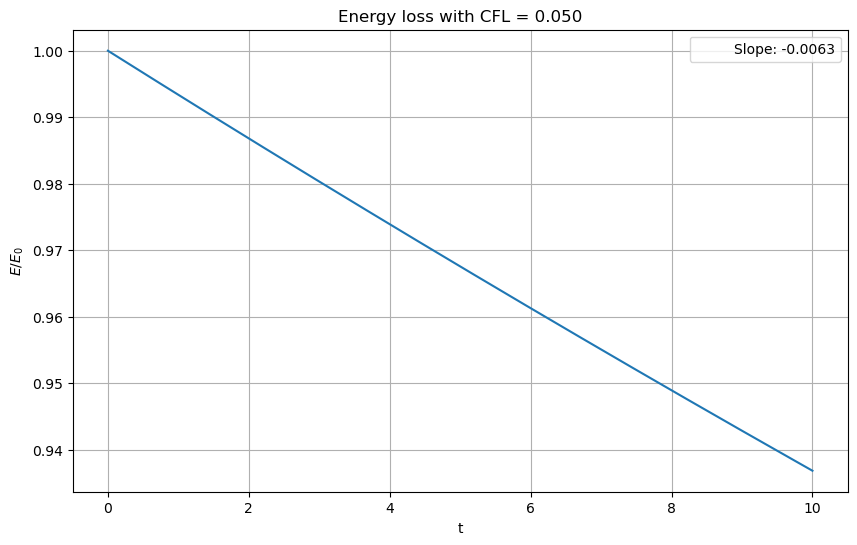
\includegraphics[width=\textwidth]{Immagini/plot-energy-decay-cfl-0.05.png}
        \end{figure}
    \end{minipage}
    \hfill
    \begin{minipage}{0.32\textwidth}
        \begin{equation*}
            \text{CFL}=0.25
        \end{equation*}

        \vspace{-0.2cm}

        \begin{figure}[H]
            \centering
            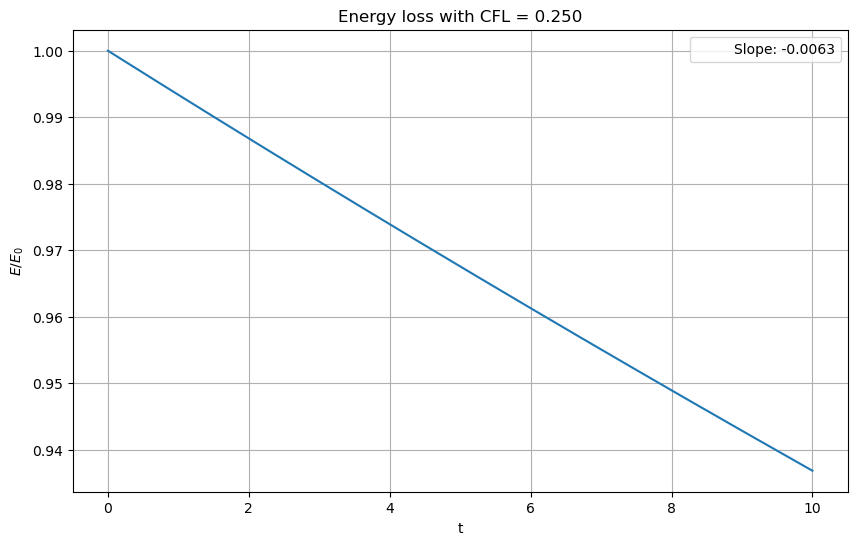
\includegraphics[width=\textwidth]{Immagini/plot-energy-decay-cfl-0.25.png}
        \end{figure}
    \end{minipage}
    \hfill
    \begin{minipage}{0.32\textwidth}
        \begin{equation*}
            \text{CFL}=0.50
        \end{equation*}

        \vspace{-0.2cm}

        \begin{figure}[H]
            \centering
            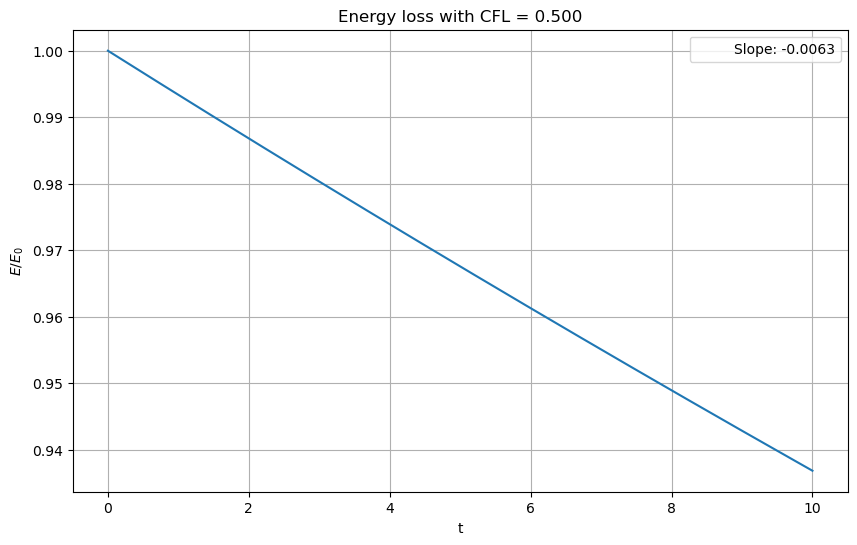
\includegraphics[width=\textwidth]{Immagini/plot-energy-decay-cfl-0.50.png}
        \end{figure}
    \end{minipage}}

    \vfill

    \footnotesize

    \pause

    Numerical energy decay is \textit{independent} of the CFL number, being entirely caused by the \textbf{implicit scheme} itself.

    \normalsize
\end{frame}

\subsection{Non-constant velocity}

\begin{frame}{What if $c=c(x)$?}
    If $c$ is not constant, its square must be interpolated as the wave function:

    \begin{equation*}
        c^2(x) \ \longrightarrow \ c_h^2(x)=\sum_{k=1}^Nc_k^{(2)}\psi_k(x)
    \end{equation*}

    \pause

    Velocity must be included in the stiffness matrix $A$:

    \begin{equation*}
        A_{i,j}=\int_0^L\left(\sum_{k=1}^Nc_k^{(2)}\psi_k(x)\right)\frac{\partial\phi_j}{\partial x}\frac{\partial\phi_i}{\partial x}dx
    \end{equation*}

    \pause

    \begin{equation*}
        \Big\Downarrow
    \end{equation*}

    \begin{equation*}
        \fcolorbox{BrickRed}{white}{\text{$\displaystyle M\frac{d^2\boldsymbol{u}}{dt^2}+A\boldsymbol{u}=0$}}
    \end{equation*}
\end{frame}

\begin{frame}{Piecewise constant velocity}
    \small

    One simple example is the \textbf{piacewise constant function}:

    \begin{equation*}
        c(x)=
        \begin{cases}
            c_1 \ \ \  &x\leqslant x_0\\
            c_2 \ \ \  &x>x_0
        \end{cases}
    \end{equation*}

    \vfill

    \alt<1>{\begin{center}
        Placing initial pulse \underline{on the left} with \textcolor{RoyalBlue}{$\boldsymbol{c_1=1}$}, \textcolor{RoyalBlue}{$\boldsymbol{c_2=3}$}:
    \end{center}

    \vspace{0.2cm}

    \begin{minipage}{0.49\textwidth}
        \begin{center}
            \textcolor{RoyalBlue}{\textbf{Dirichlet}}
        \end{center}

        \vspace{-0.3cm}

        \begin{figure}[H]
            \centering
            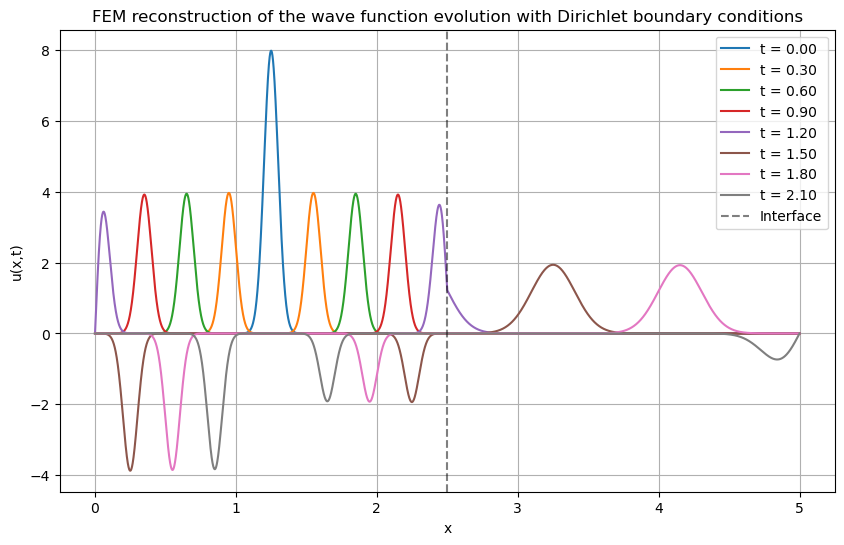
\includegraphics[width=\textwidth]{Immagini/plot-dirichlet-piecewise-c1<c2.png}
        \end{figure}
    \end{minipage}
    \hfill
    \begin{minipage}{0.49\textwidth}
        \begin{center}
            \textcolor{RoyalBlue}{\textbf{Neumann}}
        \end{center}

        \vspace{-0.3cm}

        \begin{figure}[H]
            \centering
            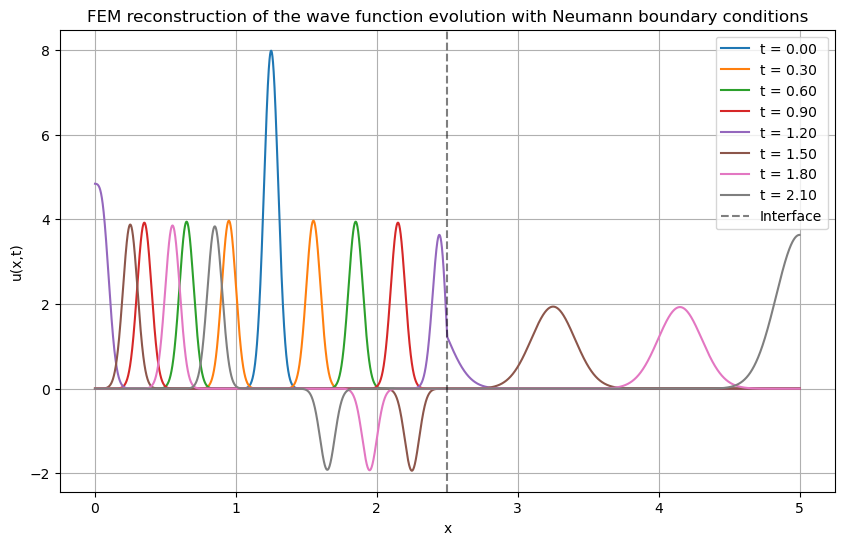
\includegraphics[width=\textwidth]{Immagini/plot-neumann-piecewise-c1<c2.png}
        \end{figure}
    \end{minipage}}{}

    \alt<2>{\begin{center}
        Placing initial pulse \underline{on the left} with \textcolor{ForestGreen}{$\boldsymbol{c_1=3}$}, \textcolor{ForestGreen}{$\boldsymbol{c_2=1}$}:
    \end{center}

    \vspace{0.2cm}

    \begin{minipage}{0.49\textwidth}
        \begin{center}
            \textcolor{ForestGreen}{\textbf{Dirichlet}}
        \end{center}

        \vspace{-0.3cm}

        \begin{figure}[H]
            \centering
            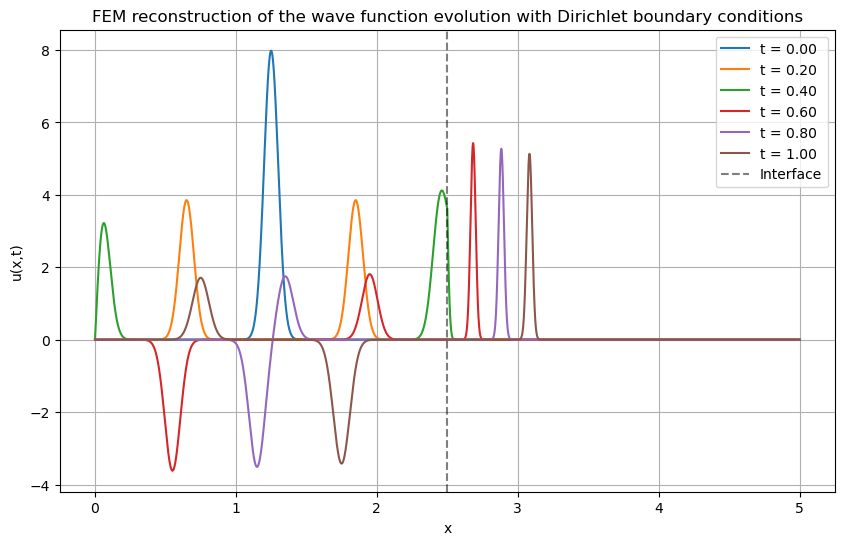
\includegraphics[width=\textwidth]{Immagini/plot-dirichlet-piecewise-c1>c2.png}
        \end{figure}
    \end{minipage}
    \hfill
    \begin{minipage}{0.49\textwidth}
        \begin{center}
            \textcolor{ForestGreen}{\textbf{Neumann}}
        \end{center}

        \vspace{-0.3cm}

        \begin{figure}[H]
            \centering
            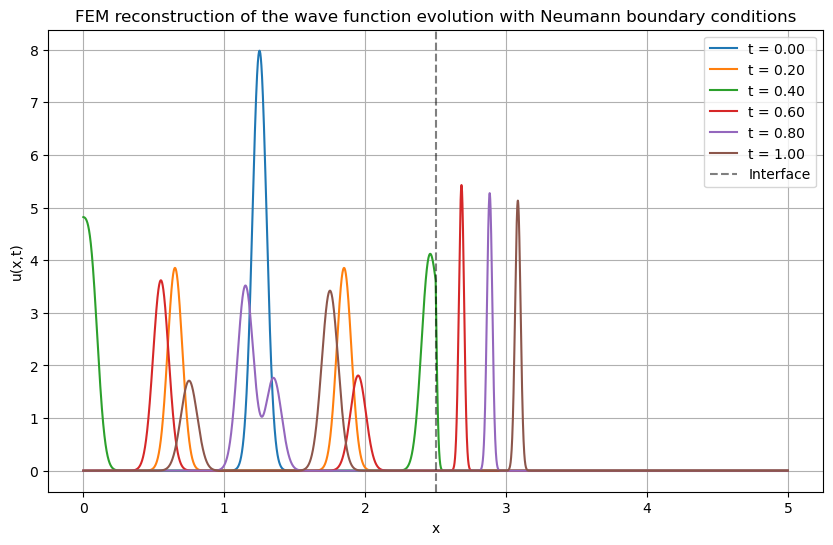
\includegraphics[width=\textwidth]{Immagini/plot-neumann-piecewise-c1>c2.png}
        \end{figure}
    \end{minipage}}{}

    \normalsize
\end{frame}

\begin{frame}{Fresnel coefficients}
    \small

    In this case, the analytical reference values are the \textcolor{BrickRed}{\textbf{Fresnel coefficients}}.

    \normalsize

    \begin{equation*}
        T=\frac{2c_1}{c_1+c_2} \hspace{1cm} R=\frac{c_2-c_1}{c_1+c_2}
    \end{equation*}

    \small

    \vfill

    \pause

    $T$ and $R$ are \underline{numerically evaluated} as the ratio of the \textbf{transmitted} and \textbf{reflected} waves to the \textbf{incident} one.

    \vfill

    \normalsize

    \visible<2>{\begin{minipage}{0.49\textwidth}
        \begin{equation*}
            \boldsymbol{\textcolor{RoyalBlue}{c_1<c_2}}
        \end{equation*}
        
        \vspace{-0.2cm}

        \begin{figure}
            \centering
            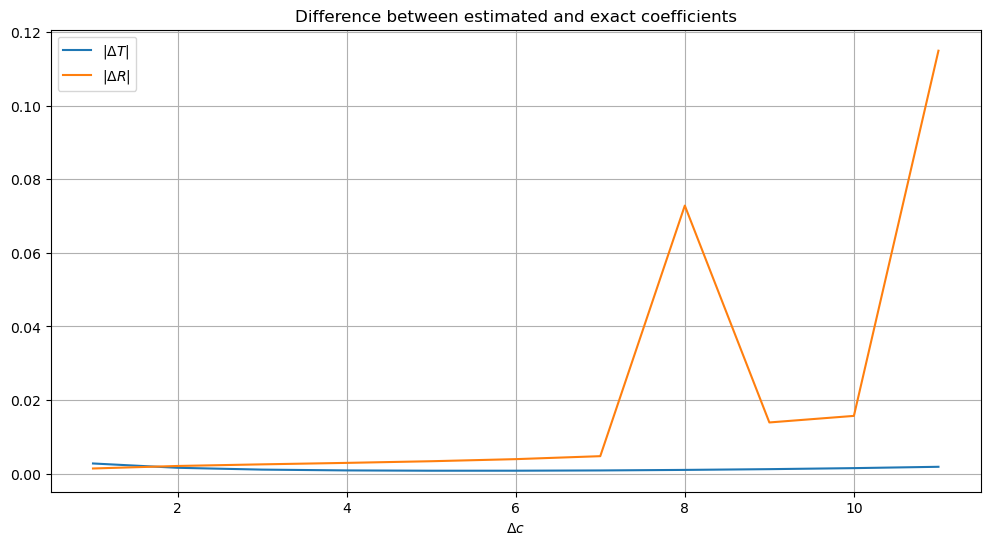
\includegraphics[width=\textwidth]{Immagini/plot-difference-coefficients-c1<c2.png}
        \end{figure}
    \end{minipage}
    \hfill
    \begin{minipage}{0.49\textwidth}
        \begin{equation*}
            \boldsymbol{\textcolor{ForestGreen}{c_1>c_2}}
        \end{equation*}
        
        \vspace{-0.2cm}

        \begin{figure}
            \centering
            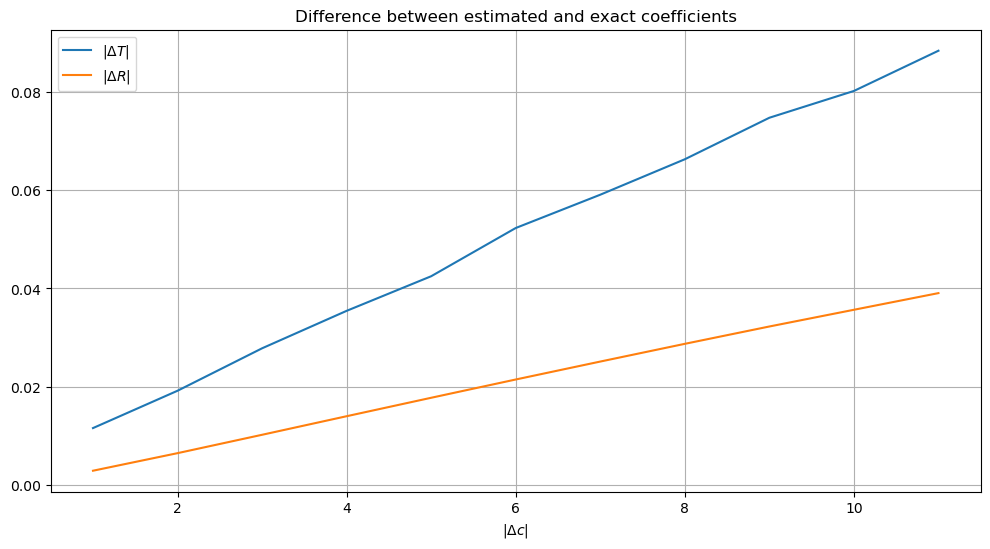
\includegraphics[width=\textwidth]{Immagini/plot-difference-coefficients-c1>c2.png}
        \end{figure}
    \end{minipage}}

    \scriptsize

    \vspace{-0.1cm}

    \begin{equation*}
        \text{Smaller velocity} \ \longrightarrow \ \text{Smaller coefficient} \ \longrightarrow \ \text{Higher sensitivity to \textbf{\underline{numerical errors}}}
    \end{equation*}
\end{frame}

\begin{frame}{Energy variation}
    Right after the wave crosses the interface, a clear \textbf{non-conservation of energy} emerges.

    \vfill

    \alt<1>{\begin{minipage}{0.49\textwidth}
        \begin{equation*}
            \boldsymbol{\textcolor{RoyalBlue}{c_1=1}} \ \ \ \boldsymbol{\textcolor{RoyalBlue}{c_2=3}}
        \end{equation*}

        \begin{figure}[H]
            \centering
            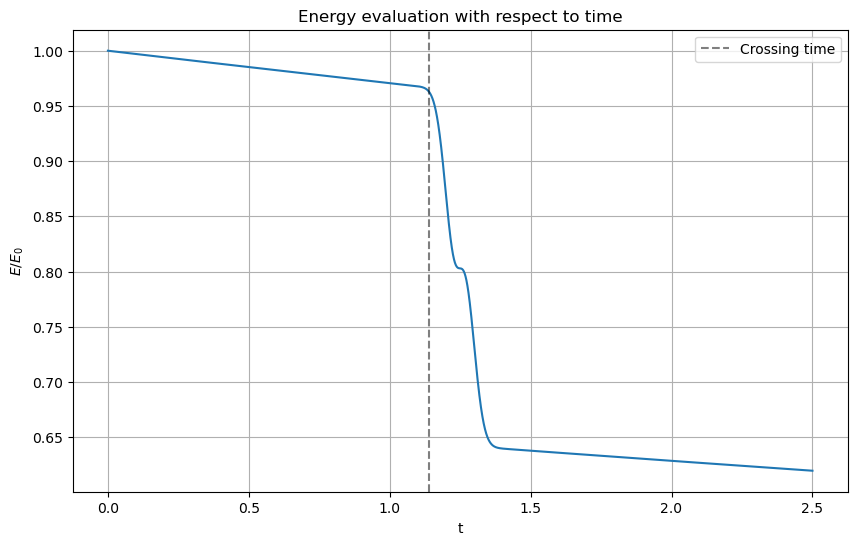
\includegraphics[width=\textwidth]{Immagini/plot-energy-c1=1-c2=3.png}
        \end{figure}
    \end{minipage}
    \hfill
    \begin{minipage}{0.49\textwidth}
        \begin{equation*}
            \boldsymbol{\textcolor{ForestGreen}{c_1=3}} \ \ \ \boldsymbol{\textcolor{ForestGreen}{c_2=1}}
        \end{equation*}

        \begin{figure}[H]
            \centering
            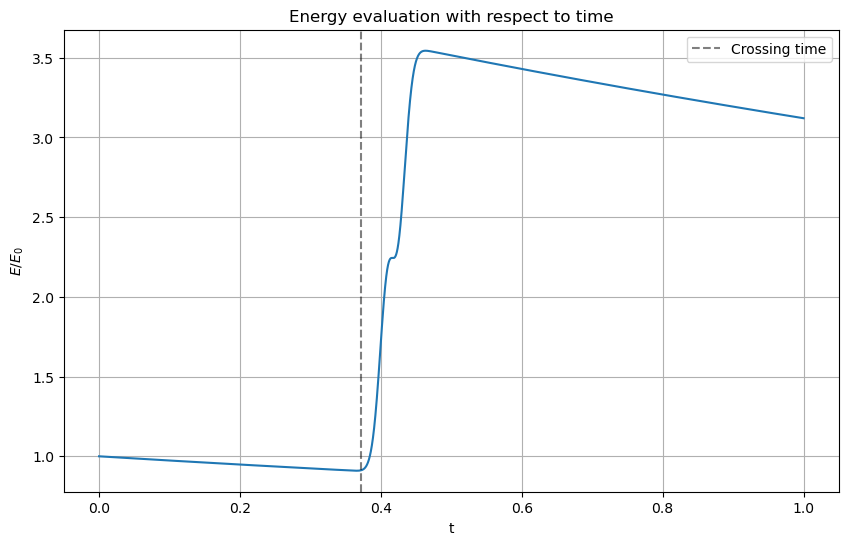
\includegraphics[width=\textwidth]{Immagini/plot-energy-c1=3-c2=1.png}
        \end{figure}
    \end{minipage}}{}

    \alt<2>{\begin{minipage}{0.49\textwidth}
        \begin{equation*}
            \boldsymbol{\textcolor{RoyalBlue}{c_1=1}} \ \ \ \boldsymbol{\textcolor{RoyalBlue}{c_2=6}}
        \end{equation*}

        \begin{figure}[H]
            \centering
            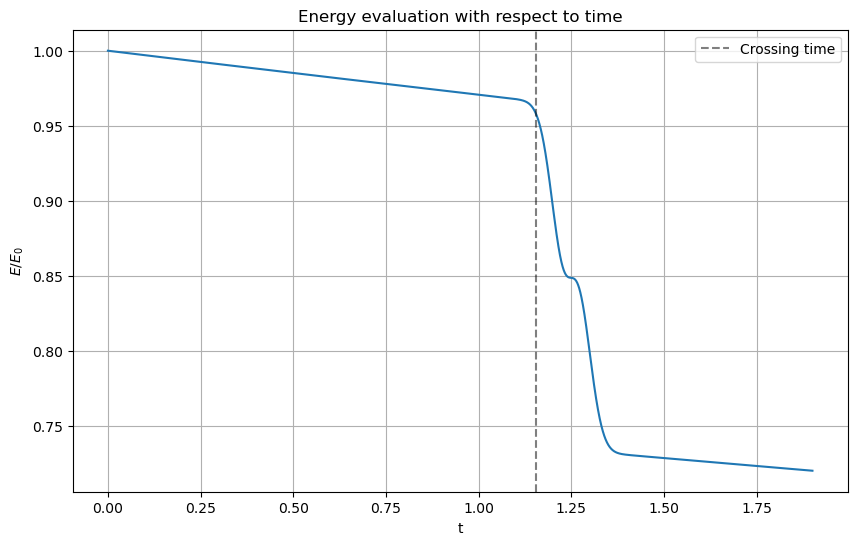
\includegraphics[width=\textwidth]{Immagini/plot-energy-c1=1-c2=6.png}
        \end{figure}
    \end{minipage}
    \hfill
    \begin{minipage}{0.49\textwidth}
        \begin{equation*}
            \boldsymbol{\textcolor{ForestGreen}{c_1=6}} \ \ \ \boldsymbol{\textcolor{ForestGreen}{c_2=1}}
        \end{equation*}

        \begin{figure}[H]
            \centering
            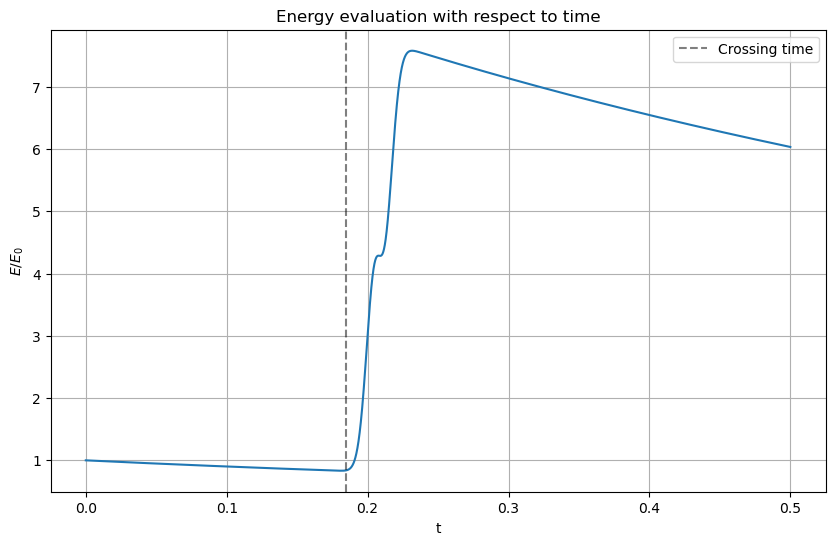
\includegraphics[width=\textwidth]{Immagini/plot-energy-c1=6-c2=1.png}
        \end{figure}
    \end{minipage}}{}

    \alt<3>{\begin{minipage}{0.49\textwidth}
        \begin{equation*}
            \boldsymbol{\textcolor{RoyalBlue}{c_1=1}} \ \ \ \boldsymbol{\textcolor{RoyalBlue}{c_2=9}}
        \end{equation*}

        \begin{figure}[H]
            \centering
            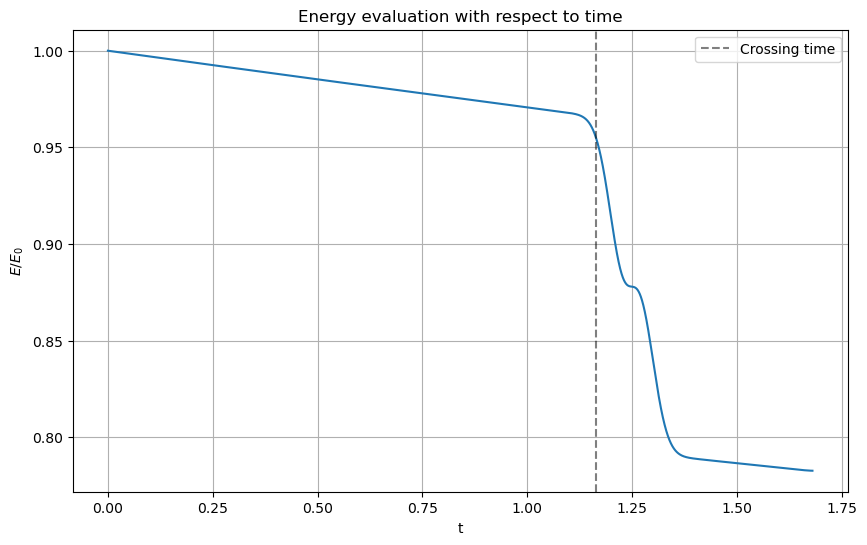
\includegraphics[width=\textwidth]{Immagini/plot-energy-c1=1-c2=9.png}
        \end{figure}
    \end{minipage}
    \hfill
    \begin{minipage}{0.49\textwidth}
        \begin{equation*}
            \boldsymbol{\textcolor{ForestGreen}{c_1=9}} \ \ \ \boldsymbol{\textcolor{ForestGreen}{c_2=1}}
        \end{equation*}

        \begin{figure}[H]
            \centering
            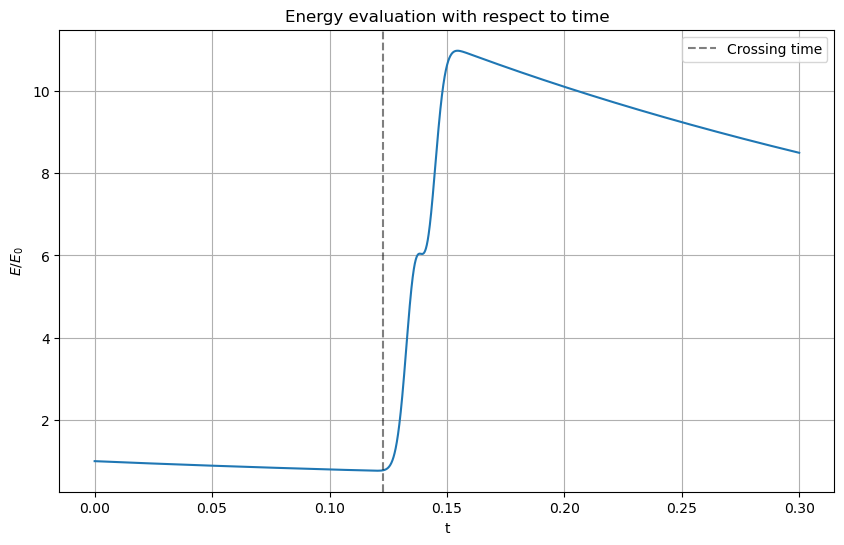
\includegraphics[width=\textwidth]{Immagini/plot-energy-c1=9-c2=1.png}
        \end{figure}
    \end{minipage}}{}

    \alt<4>{\begin{figure}
    \centering
    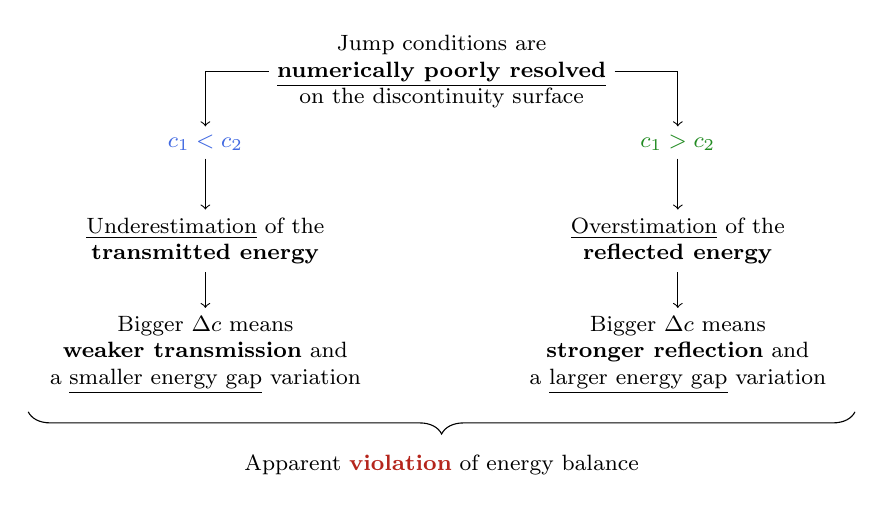
\begin{tikzpicture}
        \footnotesize

        \node[align=center] at (0,5) (A) {Jump conditions are\\ \textbf{\underline{numerically poorly resolved}}\\ on the discontinuity surface};

        \node at (-3,4.1) (B) {$\textcolor{RoyalBlue}{\boldsymbol{c_1<c_2}}$};
        \node at (3,4.1) (C) {$\textcolor{ForestGreen}{\boldsymbol{c_1>c_2}}$};

        \node[align=center] at (-3,2.85) (D) {\underline{Underestimation} of the\\ \textbf{transmitted energy}};
        \node[align=center] at (3,2.85) (E) {\underline{Overstimation} of the\\ \textbf{reflected energy}};

        \node[align=center] at (-3,1.4) (F) {Bigger $\Delta c$ means\\ \textbf{weaker transmission} and \\ a \underline{smaller energy gap} variation};
        \node[align=center] at (3,1.4) (G) {Bigger $\Delta c$ means\\ \textbf{stronger reflection} and\\ a \underline{larger energy gap} variation};

        \draw[->] (A) -- (-3,5) -- (B);
        \draw[->] (A) -- (3,5) -- (C);
        \draw[->] (B) -- (D);
        \draw[->] (C) -- (E);
        \draw[->] (D) -- (F);
        \draw[->] (E) -- (G);

        \draw[decorate, decoration={brace, amplitude=8pt, raise=2pt}] (5.25,0.75) -- (-5.25,0.75);

        \node at (0,0) () {Apparent \textcolor{BrickRed}{\textbf{violation}} of energy balance};

        \normalsize
    \end{tikzpicture}
\end{figure}}{}
\end{frame}